\section{Overview}

The test-station developped at CERN is able to automatically perform the QC tests on
up to four hybrids, either with and without the assembled and bonded pitch adapter, at the same time in a controlled environment reproducing the tracker operating temperatures. 

Despite this note mainly focuses on results of QC tests of hybrid plus PA assembly, the test station allowed to perform the first tests on bare hybrids at operating temperature, providing the first milestone validation of the mechanical and electrical design of the hybrid circuit.

The hybrid test station was planned to perform QC test on the entire or a consistent fraction of the $\sim$18000 hybrids to be assembled over a period of .... For this reason the test station design guidelines are based to get a throughput of while ensuring safe testing and handling conditions.

A simplified functional scheme of the test-station can be seen in Figure~\ref{fig:teststation_scheme}. A labeled  picture of the setup is visible in Figure~\ref{fig:setup}.

\begin{figure}[h]
  \begin{center}
    \resizebox{\textwidth}{!}{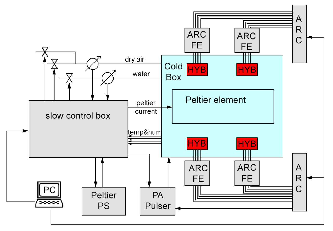
\includegraphics{fig/teststation_scheme_small.pdf}}
    \caption{Functional scheme of the hybrid teststation}
    \label{fig:teststation_scheme}
  \end{center}
\end{figure}

\subsection{DAQ}

The hybrids are read out by ARC boards in combination with the old version of the ARC front-end adapter.

\clearpage

% \begin{2figures}{t}
%   \resizebox{0.46\textwidth}{!}{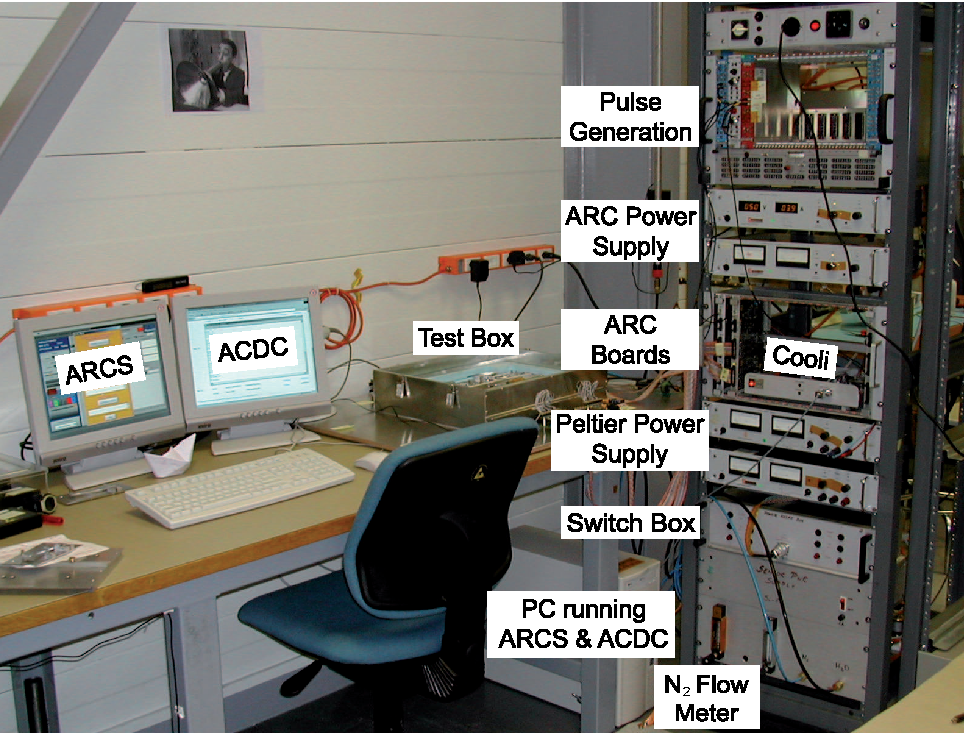
\includegraphics{fig/setup_labels.pdf}} &
%   \resizebox{0.46\textwidth}{!}{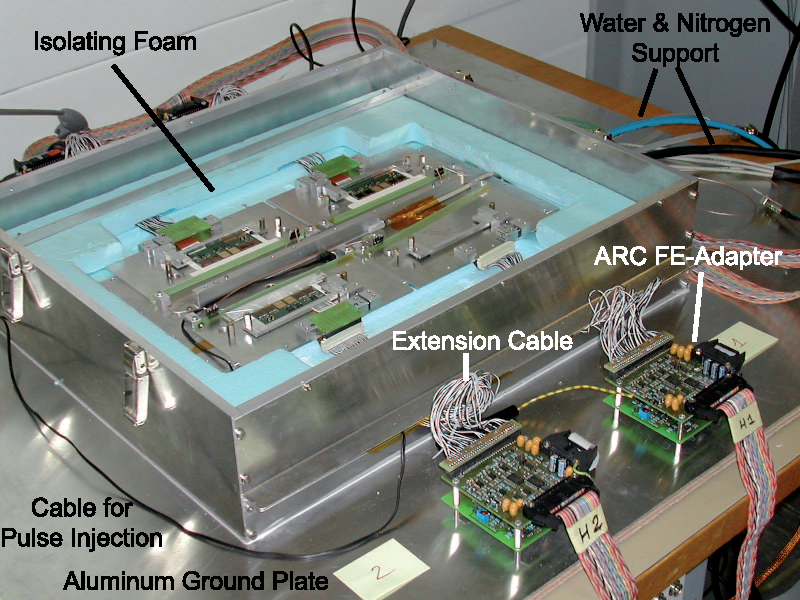
\includegraphics{fig/climatic_chamber_labels.pdf}} \\
%   \caption{The test-station setup at CERN.}
%   \label{fig:setup} &
%   \caption{The test-station climatic without the cover lid; three of
%   the four slots are occupied by hybrids.}
%   \label{fig:climaticchamber} \\
% \end{2figures}
\begin{figure}[t]
  \begin{center}
    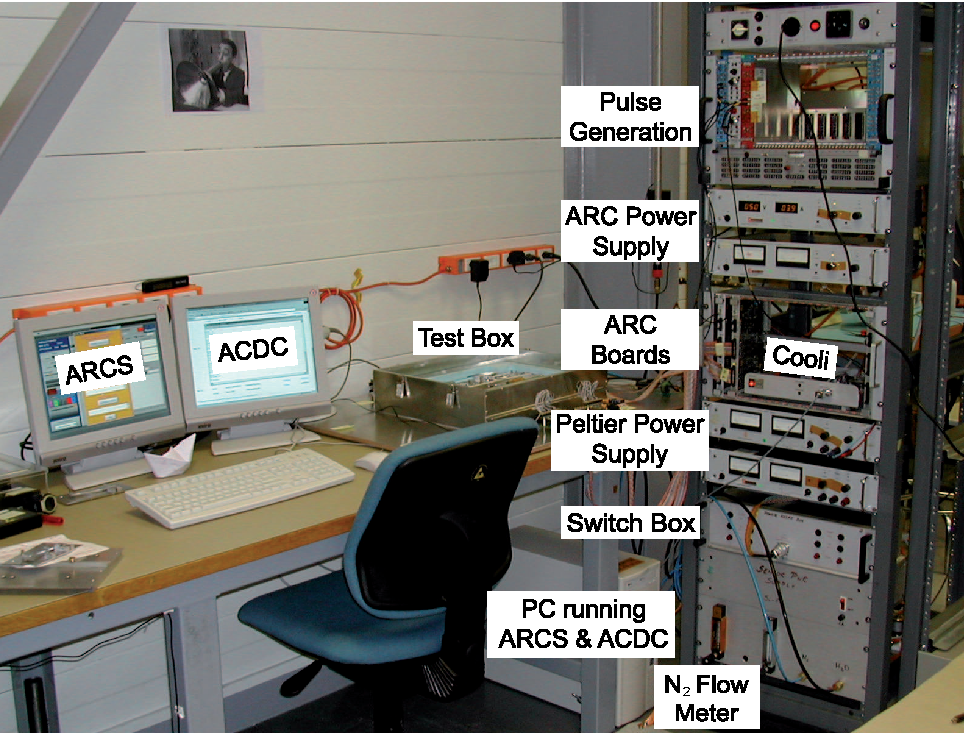
\includegraphics[width=0.8\textwidth]{fig/setup_labels.pdf}
    \caption{The test-station setup at CERN.}
    \label{fig:setup}
  \end{center}
\end{figure}
\begin{figure}[b]
  \begin{center}
    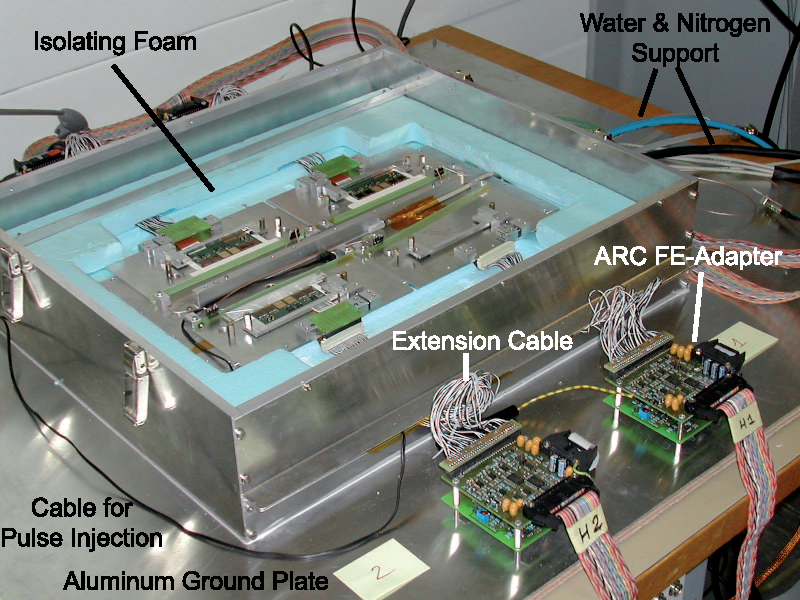
\includegraphics[width=0.8\textwidth]{fig/climatic_chamber_labels.pdf}
  \caption{The test-station climatic without the cover lid; three of
  the four slots are occupied by hybrids.}
  \label{fig:climaticchamber}
  \end{center}
\end{figure}

\clearpage

\subsection{Climatic chamber}

The main component of the test-station is the climatic chamber or {\em cold-box}. It is a thermally-insulated aluminum box suited to host up to four hybrids of any kind\footnote{There are 26 different kinds of hybrids that could differ either for the bare hybrid kind and for the different PA.}. The throughput depends either on the possibility to test in parallel up to four hybrids but also on the rapid thermal cycles, achieved thanks  to the limited volume, the low material budget and the good isolation and to the powerful active element and\\
The climatic chamber is visible in Figure~\ref{fig:climaticchamber} without the cover lid.  When closed, the overall internal dimensions of the box are roughly $\sim 45\times 38 \times 11 \cm ^3$. For shielding purposes the box is entirely made of aluminum, 1cm thick for the lateral walls, 2mm thick for the bootom plate and the removal cover lid. The bottom plate extends well beyond the box itself to host the readout electronic boards and is screw-tightened to a 2cm thick plywood board to be sufficiently stiff. 

The box portion actually under temperature control is a $37\times20\times2\cm^3$ volume defined by two aluminum cooling plates: the bottom one, $6\mm$ thick is screw-tighttened to the 'cold' side of the Peltier element sitting underneath; the top one, $2\mm thick$ is screw-tighttened to a longitudinal $\sim30\times1\times2\cm^3$ aluminum beam sitting on the bottom plate. In such a way also the top plate is in good thermal contact with the cooling element to guarantee an uniform heat removal. The top plate must be removed for the hybrid loading.

The remaining part of the box is essentially occupied by thermal-insulating foam in which the peltier element and also all needed services are buried. The top part of insulation must also be removed for hybrid loading. Box walls are thermally insulated by at least $30\mm$ of foam-like material.

The Peltier element\footnote{Supercool AB Sweden, model DL-290-24-00.}  has a rectangular shaped $220\times55\mm^2$cooling surface of and is capable of 290W max cooling effect (24V - 14A). It allows the operating temperature of the hybrids to be set in the range between -25$^\circ$ and $40^\circ$ in case of maximum heat load (four 6APV fully working hybrids, i.e. $\sim 0.1W/$channel$\times768$channels$\sim$80W). Heat is removed from the 'hot' side of the peltier element by the built-in cooling cicuit in which $\sim$4 l/min (?) flux of room temperature tap water are circulated in standard operating conditions.

The hybrids are delicate to handle because of non protected bonds on the circuit surface. A safe and easy loading is achieved by hosting each hybrid on a removable aluminum support plate that, for optimal thermal coupling, has to be screw-tightened on the bottom plate. The support plate features also a robust clamp to ensure a good and uniform contact with the hybrid ceramic substrate. The hybrid pig tail features a Nais miniaturised connector with a life of only few tenths of insertions and removals, a figure not far from the number of times that the hybrid has to be connected for testing purposes for hybrid QC first and then also for module QC. For this reason, each hybrid is equipped with a card to adapt the Nais connector to a more robust Samtec connector since the first tests at the company until the final installation of the module. A spring loaded mechanism is implemented to hold this adapter card to avoid unwanted stress on the hybrid pigtail. A TOB bare hybrid on the support plate is visible in Fig.~\ref{fig:hybrid_on_support_plate}.
\begin{figure}[hbt]
  \resizebox{\linewidth}{!}{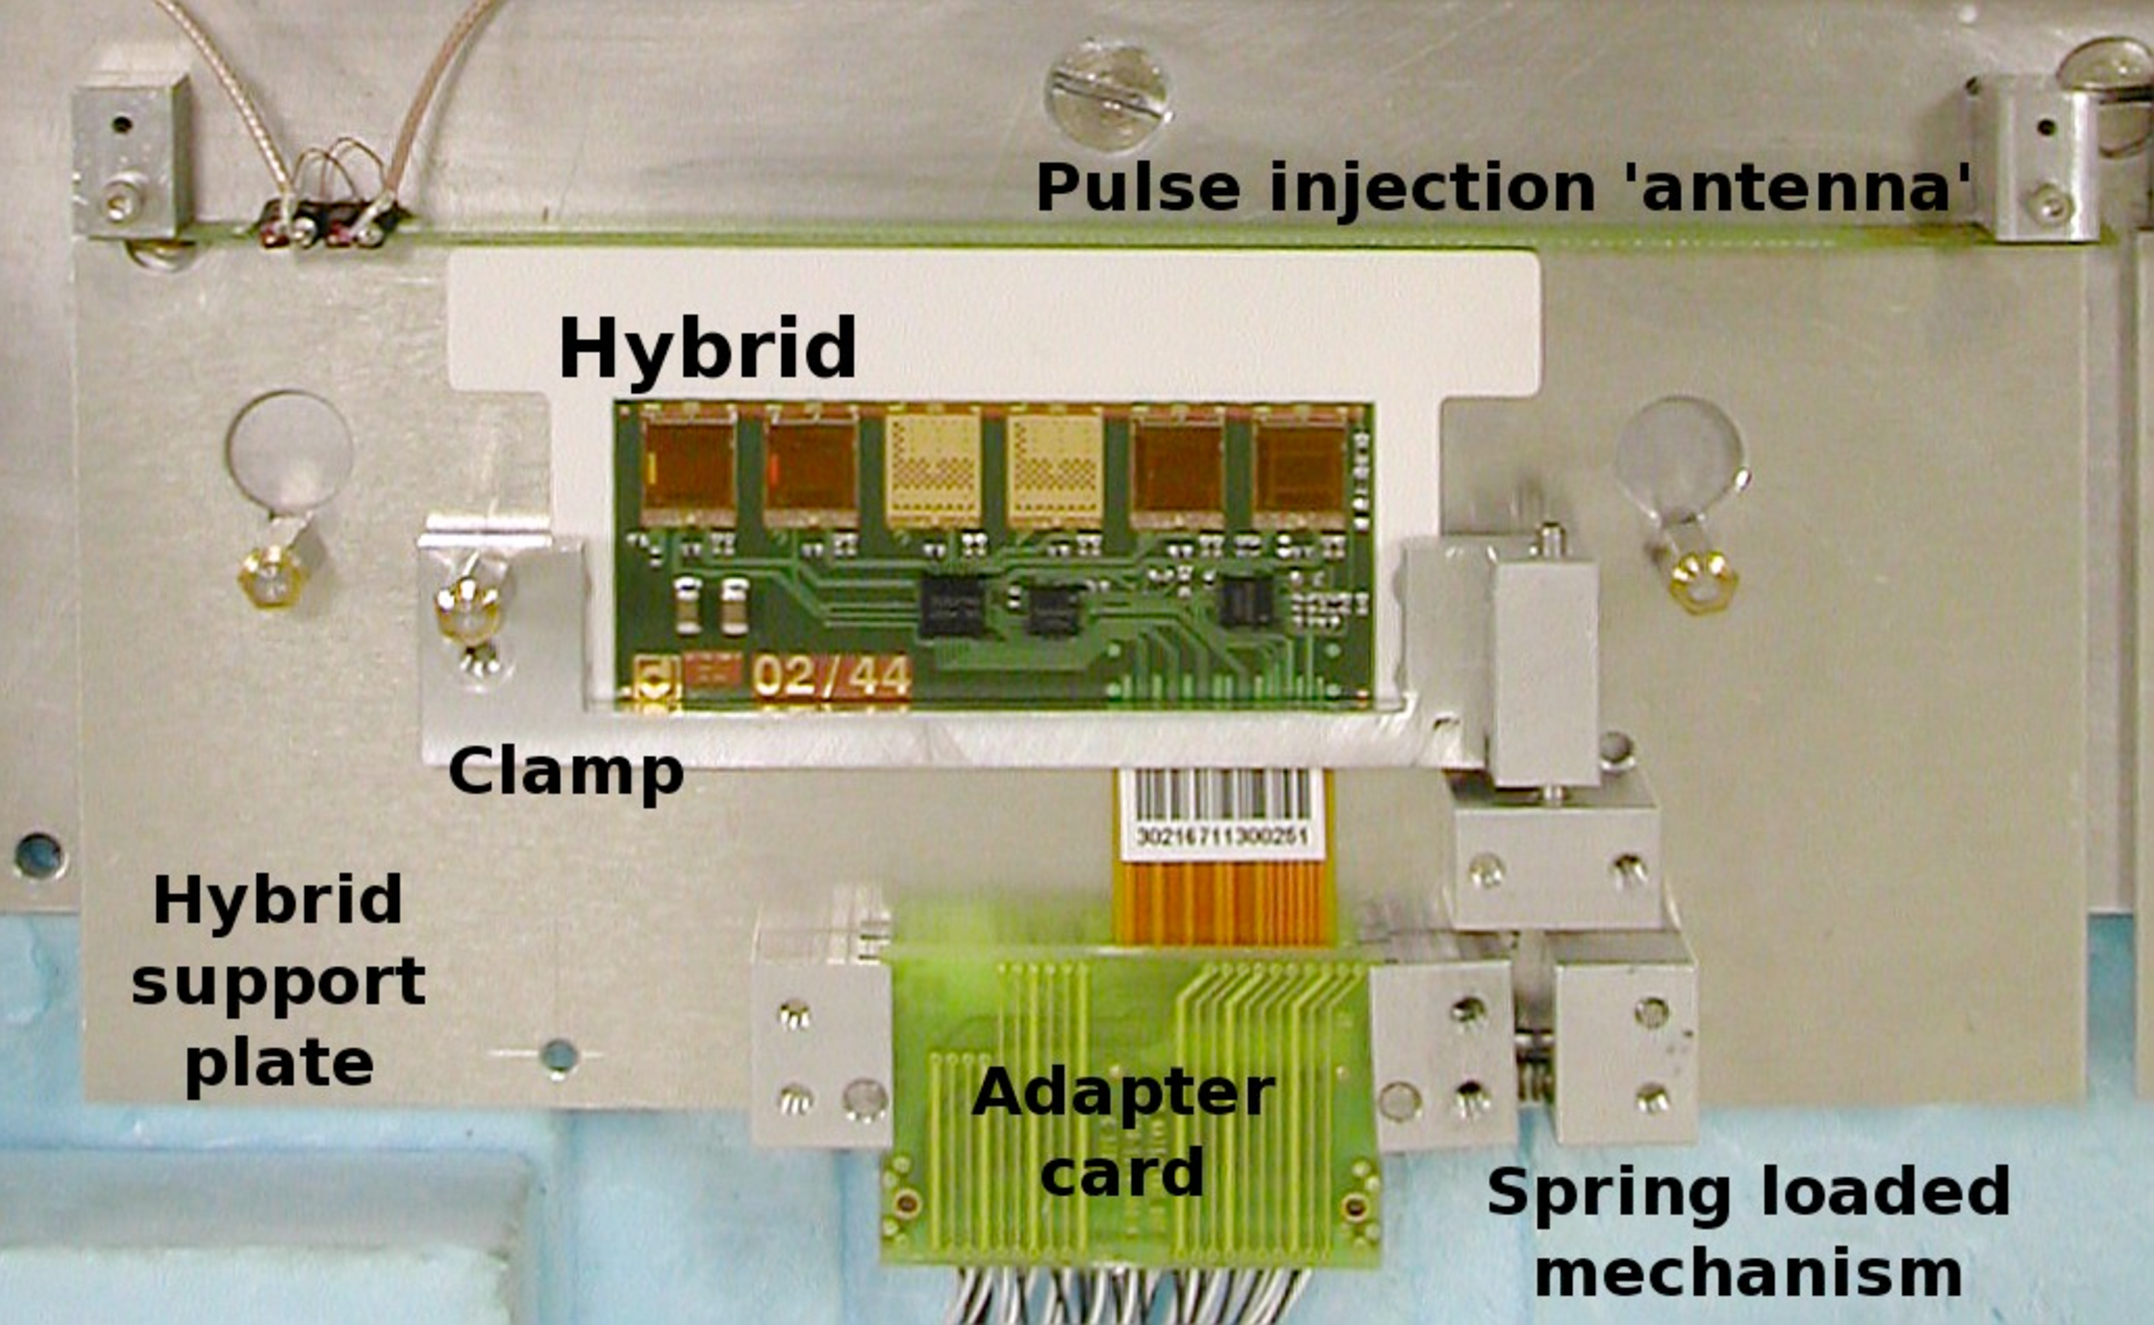
\includegraphics{fig/hybrid_on_support_plate.pdf}}
  \caption{Photograph of a hybrid (without pitch adapter) mounted on a support plate. The plate simplifies the mounting procedure as it provides a handle far off the fragile bonds on the circuit.}
  \label{fig:hybrid_on_suport_plate}
\end{figure}


The cold box can be flushed with nitrogen or dry air to avoid water condensation at the lowest temperatures. To minimize the gas flow the cold box as been carefully made as much gas-tight as possible.

\subsection{Environmental control and monitoring}

The temperature and the humidity are monitored by the cooli box (see section \ref{sec:cooli_box}) which is interfaced by a CERN special version of ACDC (see also \ref{subsection:hybrid_test_station_software}).\\

The control and monitoring of the climatic chamber relies on a versatile slow control board called {\em cooli box} and designed in (where?)~\cite{cooli}. It is based on a programmable microcontroller and the capability to monitor temperatures and humidity and to control the peltir eement rely on the following features:
\begin{itemize}
\item RS232 interface for PC remote control;
\item analog inputs: eight 10-bit, 0-5V ADC; they can be used for any kind of voltage output sensors (like humidity sensors or flow meters);
\item analog outputs: four 10-bit DAC, two 0-5V, two 0-10V;
\item specialized input for the Dallas DS1820 digital thermometers, that can be put in series on a single 3-wire bus (data, ground, +5V); 
\item switch for the control of the polarity of the Peltier element power supply.
\end{itemize}

The performance of tests in a temperature reduced environment necessitates the careful monitoring and control of the humidity because condensation of water is very likely when the temperature is reduced by 40�C.  A humidity sensors of type hih3610 from Honeywell~\cite{bib:hih3610} is placed in the test volume for humidity measurement. The sensors provide an analog voltage output which is connected to the analog input of the cooli box.
The humidity is actively controlled by a switch box that hosts four independent electro-valves that can be driven by the DAC output of the cooli box. The simple but effective configuration of the gas circuit sketched in Fig.~\ref{fig:gas_flow} allows a rather stable control of the humidity in the cold box. The dry air or nitrogen line feeds in parallel two valves, each one followed by a standard gas flow regulator: one being set to a {\em high flow} of $\sim 200$l/h, the other set to a {\em low flow}, $\sim 10$l/h . Depending on the humidity measurement and on the test phase, the software decides if and which of the two branches needs to be opened. The relative humidity is always kept below 30~\% during operation.\\
\begin{figure}[h]
  \begin{center}
    \resizebox{\textwidth}{!}{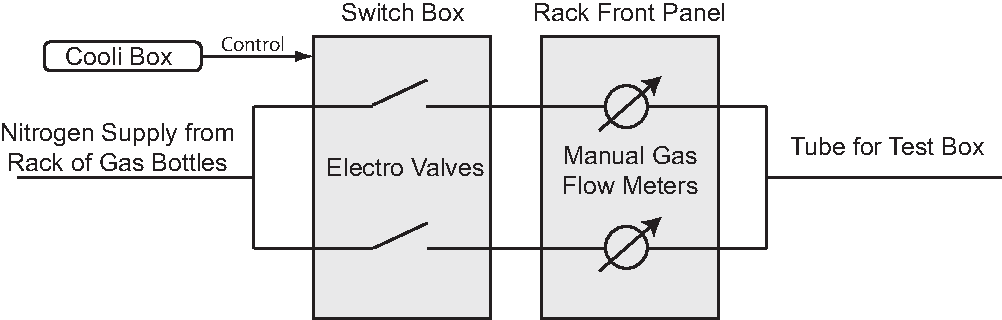
\includegraphics{fig/hybrid_test_station_gas_flow}}
    \caption{Functional scheme of the hybrid teststation}
    \label{fig:gas_flow}
  \end{center}
\end{figure}


The temperature of the hybrids is measured by four DS18B20 sensors from Dallas Semiconductor~\cite{bib:dallas_sensor} sitting just below each hybrid support plate, but thermally decoupled from the cold box bottom plate.\\

Temperature is controlled by the heating/cooling power of the peltier element. The peltier element supply current is provided by an analog programmable power supply\footnote{Delta Elektronika BV, SM 7020-D.}. In such a device the output current is proportional to the 0 to 5V voltage applied at the programming analog input. This input is driven by one of the DAC outputs of the cooli box. The cooli box also features a relay based switch to polarity of the current flow into the peltier element. The DAC setting and the current direction is calculated by the slow control software ACDC as described (\ref{sec:slowcontrol}). One of the electro valves of the switch box is used to switch the water for the peltier element on and off. The remaining one could be used as spare.\\

%Current...\\
%PID algorithm...\\

\subsubsection {Safety (to be reviewed)}
Next to the temperature and humidity range warnings which are described in section~\ref{sec:acdc} and the cooli interlock two sensors are implemented in the hybrid test station for the detection of operation failures. They are very useful to check if the test station is provided with the necessary water and nitrogen supply. Both sensors are monitored via the analog inputs of the cooli box. Thus they are software implemented.\\
An electrical self made gas flow detector is used to monitor the gas flow. This feature is useful as the manual flow meters provide only optical information when the gas supply rack is empty. The resistivity difference between a pair of identical thermocouples is converted to a temperature difference information. One of the thermocouples is fixed inside the gas supply tube while the other is fixed outside the pipe to provide reference information. When gas is supplied to the test box the sensor inside the tube cools down to the nitrogen temperature while the reference probe heats up. The resistivity difference is converted to a voltage information which is displayed by the software and if necessary initiates an alert.\\
A water flow sensor is connected to the water supply to check if the water tap is on or off.\\

\subsubsection{Shielding and Grounding Issues}
The pitch adapter lines can pick up spurious signal sources since a grounding plane is not present underneath as for the rest of the hybrid. While this feature is useful for intentional signal injection it is counterproductive for the determination of the hybrid noise if external noise sources are present. A reliable measurement of noise is only possible if a grounding and shielding scheme is implemented which avoids the transfer of noise into the APV. The effect a proper grounding and shielding scheme has is shown in figure \ref{fig:hybpa_influence_shielding}.\\
\begin{figure}
  \begin{center}
    \resizebox{\textwidth}{!}{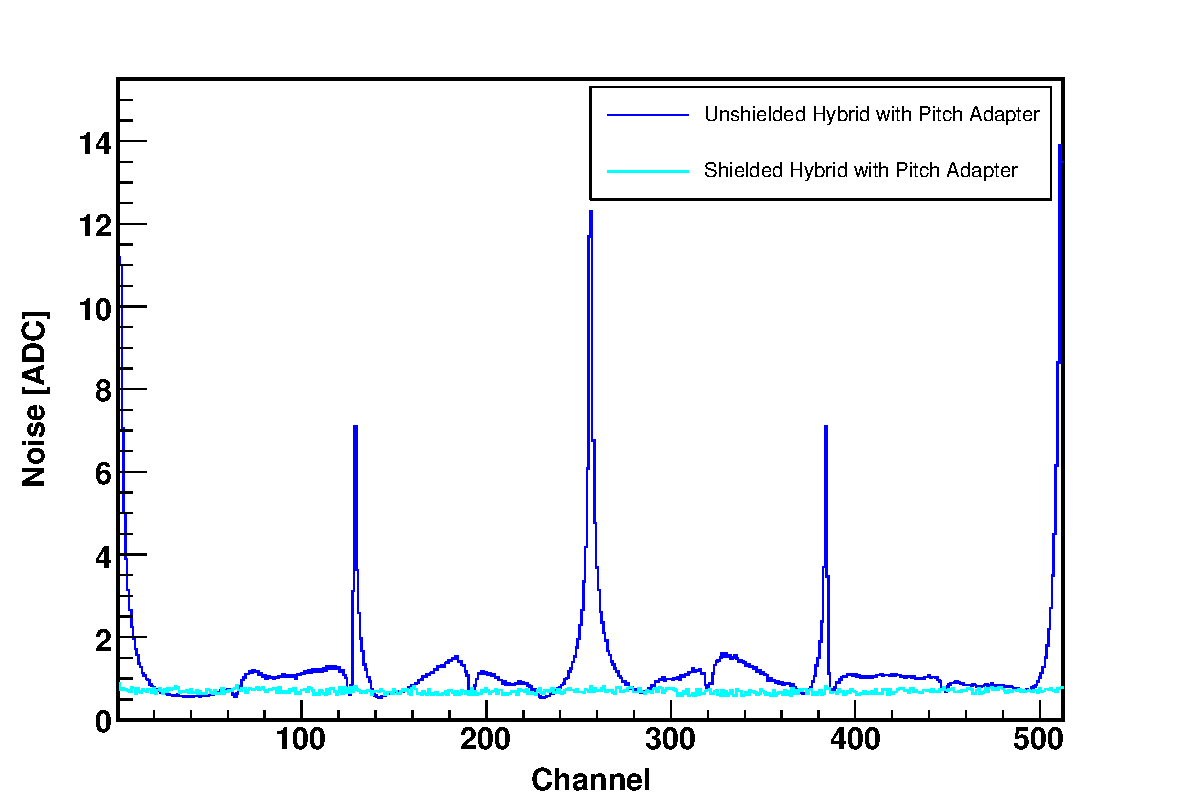
\includegraphics{fig/c1_hybpa_noise_shield_comparison.pdf}}
\caption{The noise of an unshielded hybrid with pitch adapter compared with the noise of a hybrid with pitch adapter which was tested inside the test box.}
\label{fig:hybpa_influence_shielding}
  \end{center}
\end{figure}

Shielding is provided by the test box. When the hybrids are under test the test box is closed thus they are completely surrounded by aluminum.\\
Since the ARC power supplies are floating, the natural ground reference would be given by the PC via the 50 pin flat band cable that interfaces the ARC board on one side and the PCMIO PC card on the other. Unfortunately the implementation of a traditional 'star' grounding configuration where the ground is distributed from a common point carefully avoiding ground loops did not give good results, probably because fast signals are involved and it is very difficult to make ground connections with sufficient low impedence. In the case of the hybrid test station, distributed ground connections were found to be fundamental to minimize spurious signal injection in APV inputs. In particular it turned out to be crucial to connect the local hybrid ground to the hybrid support plate to which the capacitive pitch adapter lines coupling is maximal. The grounding scheme of the hybrid test station is shown in figure \ref{fig:grounding_test_station}.
\begin{figure}
  \begin{center}
    \resizebox{\textwidth}{!}{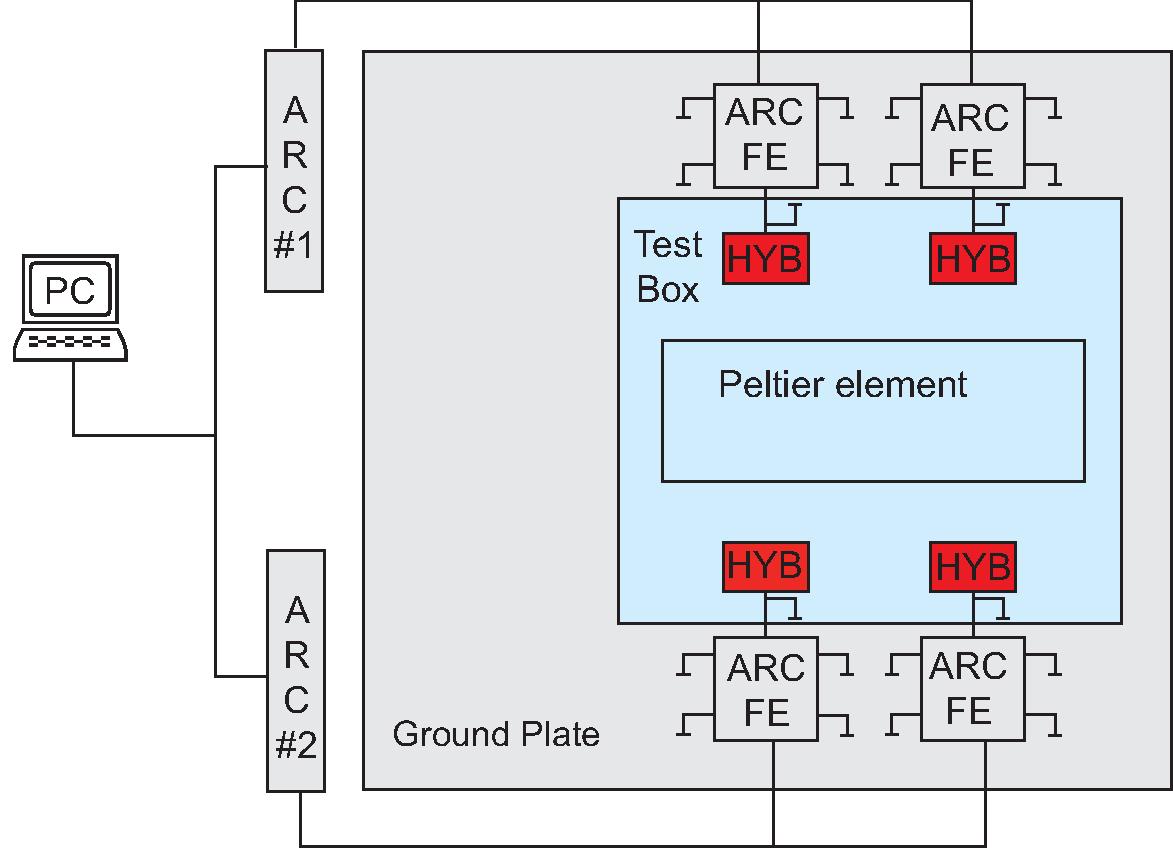
\includegraphics{fig/grounding_scheme_test_station.pdf}}
\caption{The grounding scheme of the hybrid test station.}
\label{fig:grounding_test_station}
  \end{center}
\end{figure}

\section{Finding shorts}
\subsection{Principle}

When the input of two channels are shorted, any signal at the input of
one of them will be split up between both. When using the internal
calibration facility of the APV chip, signal is applied on every 8th
channel. This means that the two neighbouring inputs of the probed
channel should not get any signal. If there is a short to one of the
neighbours, the signal is split up and decreases significantly in
height. A short can thus be found by applying a cut on the calibration
signal height. 

\subsection{Description}
To detect the shorts we perform a calibration run in peak mode with
the inverter off. The calibration charge that is injected into the
amplifier inputs is roughly corresponding twice the charge that a MIP
generates in a $300\um$ silicon sensor. The latency is chosen such that
the sampling occurs at the pulse maximum. The expected signal is
around 70 ADC counts and a signal less that 50 ADC counts is
considered a short (see fig.\ref{fig:shorts}). 

\begin{figure}[hbt]
  \resizebox{\linewidth}{!}{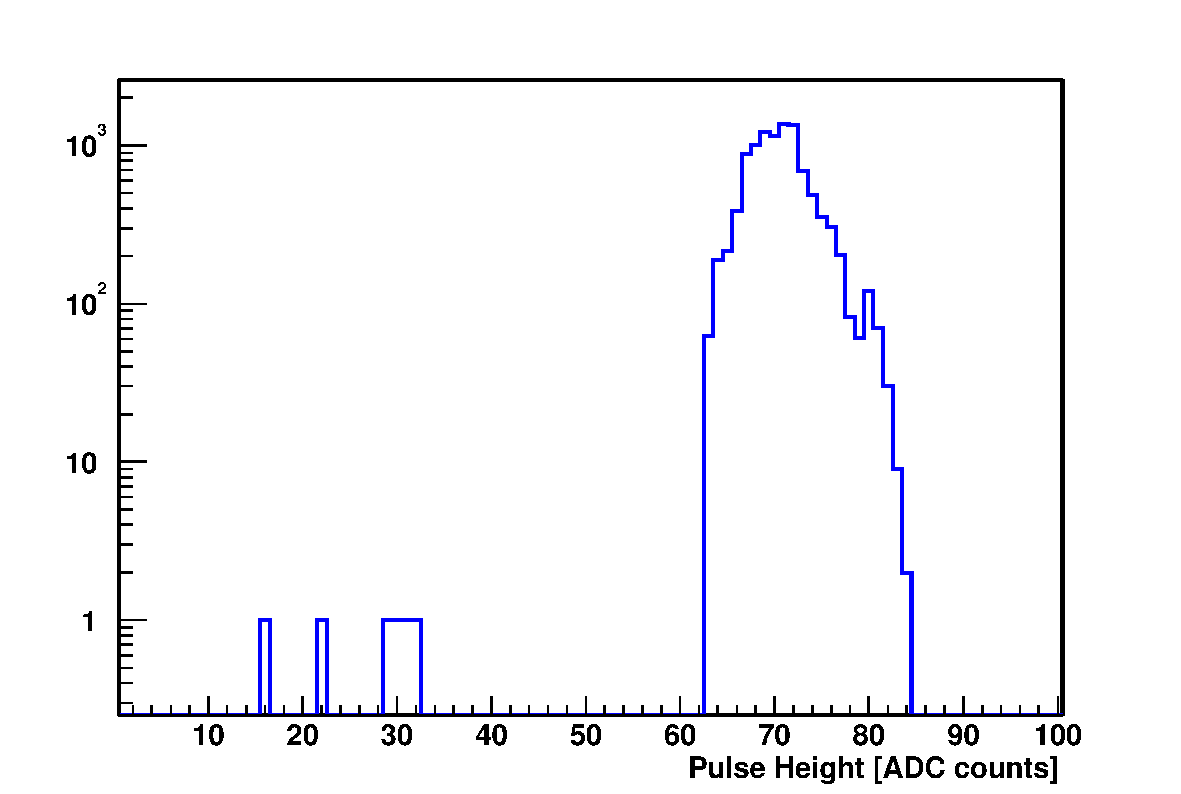
\includegraphics{fig/shorts.pdf}}
  \caption{Pulseheight distribution for all 512 channels of 21 hybrids.}
  \label{fig:shorts}
\end{figure}

\section{Finding opens}
\subsection{Principle}

To find opens, a signal is injected through capacitive coupling into
the pitch adapter lines. Since all channels on the hybrid see
simoultaneously a charge at their inputs, the on-chip common mode
subtraction of the APV tries to compensate for it, resulting in a more
or less flat output at the end of the shaper stage. If one of the
APV-pa bonds is lifted, or if a pa line is broken, no signal is
present on that channel, and the common mode subtraction will make it
stick out sharply with respect to its neighbours. 

\subsection{Description}

The signal injection system, shown schematically in Fig.~\ref{fig:signal_injection_pa}, uses the logical OR of the trigger LVDS signals from the two ARC boards.  Some intermediate conversions are needed to be able to use off-the-shelf NIM modules. A timing unit is used to regulate the signal duration. Finally,
the injected signal is obtained by the positive edge of the trigger signal, converted to TTL to have enough signal strenght, and applied on a $50\Omega$ terminated  wire brought closely to the sensor side of the pitch adapter and acts like an 'antenna'. The pulse synchronization is achieved by choosing a proper APV latency.  During normal operation the cooli box disables the pulse injection.\\
\begin{figure}[htbp]
  \resizebox{\linewidth}{!}{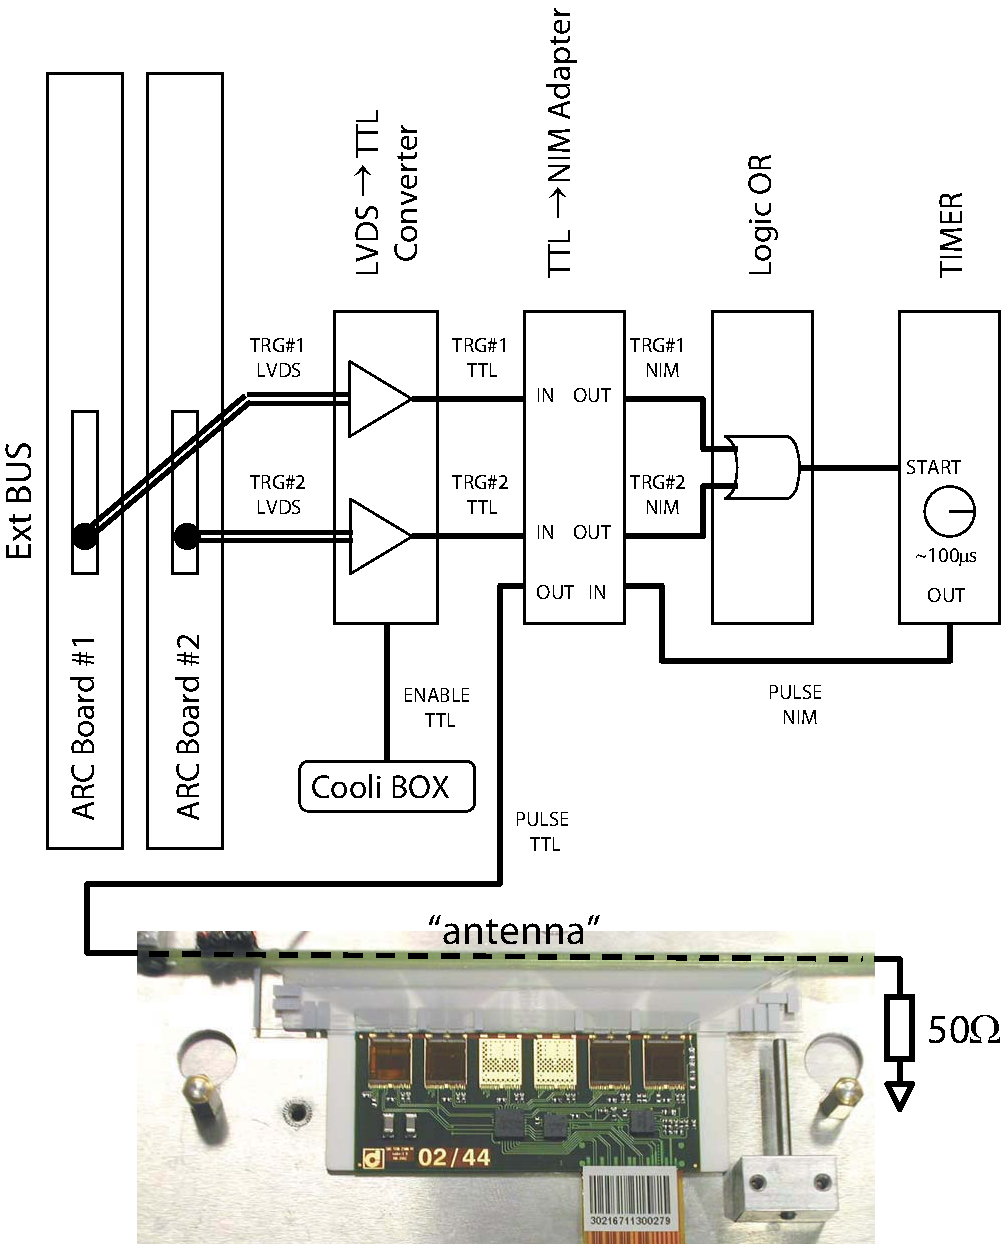
\includegraphics{fig/pulser.pdf}}
\caption{The scheme of signal injection on the pitch adapter of a hybrid. The APV trigger on the expansion bus of the ARC board is used to initiate TTL pulses which induce a signals into the pitch adapter lines.}
\label{fig:signal_injection_pa}
\end{figure}

The capacitive coupling is mostly going to the bond pads, so
that it even becomes possible to detect broken pa lines that are open
close to the bond pads. The pedestal is measured in peak mode with the
inverter stage off. For a hybrid without faults the result is a more
or less smooth pedestal distribution (see fig.\ref{fig:opens} a)). 
The pedestals at the edges of the APV chips are pulled downwards.
The result of a hybrid with open bonds and broken pa lines is shown in
fig.\ref{fig:opens} b).
The faulty channels stick out as positive spikes from the rest.
\begin{2figures}{hbtp}
  \resizebox{0.45\textwidth}{!}{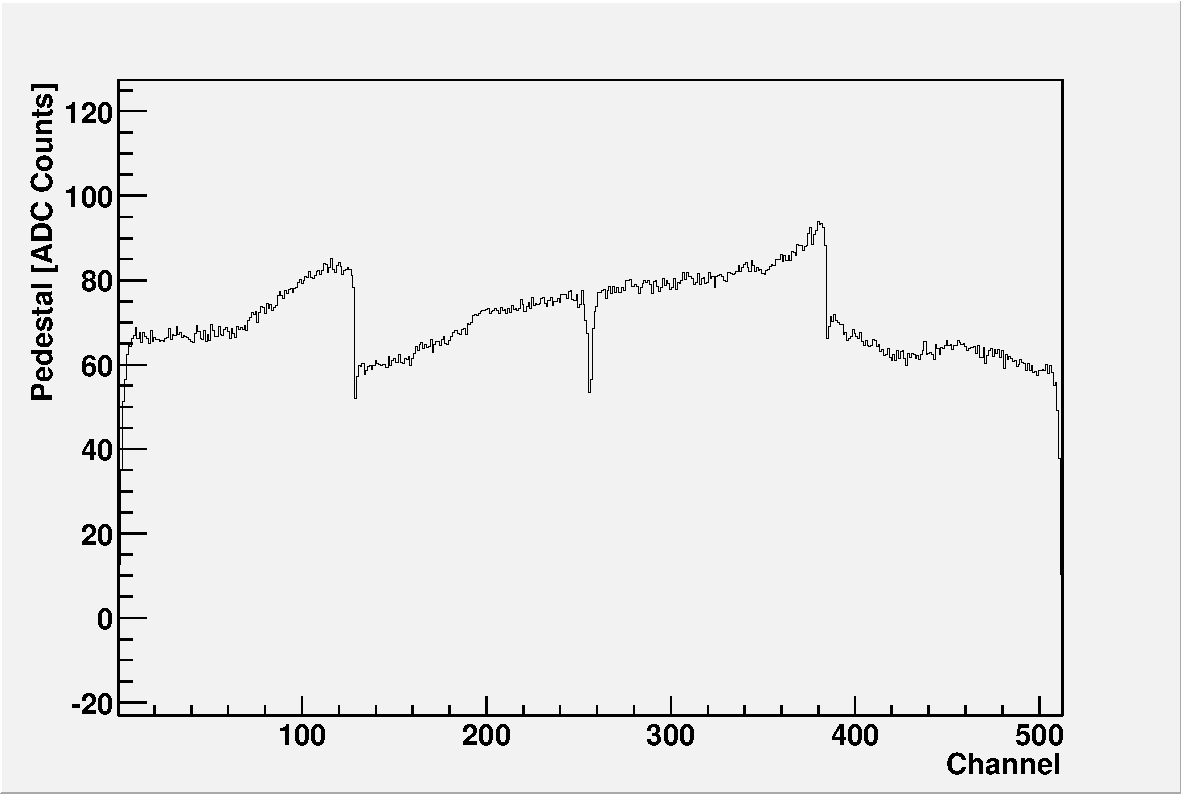
\includegraphics{fig/noopens.pdf}} &
  \resizebox{0.45\textwidth}{!}{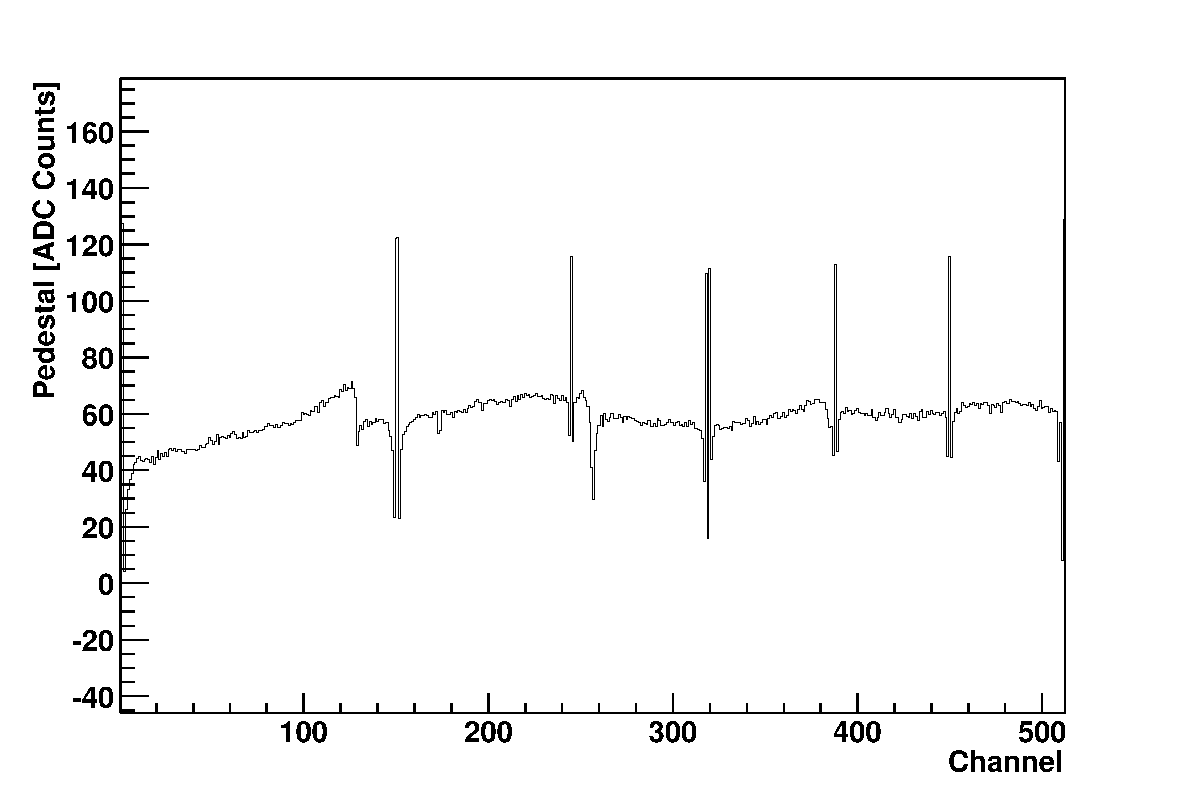
\includegraphics{fig/opens.pdf}} \\
  \caption{Pedestal distribution with signal injected into the pitch
  adapter for a hybrid with no opens.}
  \label{fig:noopens} &
  \caption{Pedestal distribution with signal injected into the pitch
  adapter for a hybrid with n opens.}
  \label{fig:opens} \\
\end{2figures}

A naive approach to find opens by applying an absolute cut on the
pedestal values does not work, because the average pedestal values can
vary considerably from chip to chip. We therefore have to subtract the
average pedestal value chip-wise. Still the slope in the pedestal
distribution of a single chip, which is due to imperfect capacitive
coupling to the signal wire, makes it sometimes difficult to apply a
single cut on these values. To cope with this we also consider the
difference of a pedestal values to its neighbours. 
Fig.\ref{fig:scatter} shows a scatter plot of the average-subtracted
pedestal values against the difference to the neighbours. 
The faulty channels group in the top right corner. We use a straight
line to separate them from the bulk of good channels that is also
shown in the figure giving raise to the following condition for bad
channels: 
\begin{displaymath}
  y-a\cdot x>b
\end{displaymath}
where the slope $a=$-0.1 and the abscissa $b=$45 ADC counts.
\begin{figure}
  \resizebox{\linewidth}{!}{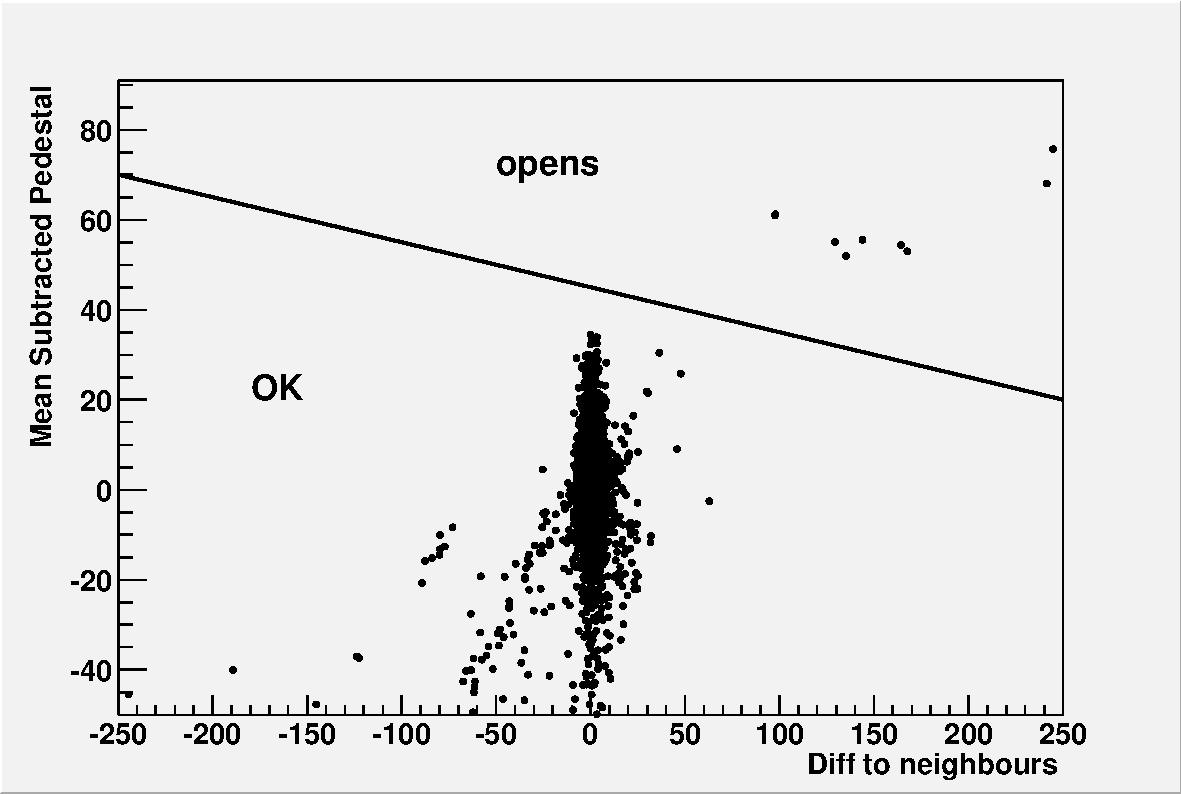
\includegraphics{fig/scatter2.pdf}}
  \caption{}
  \label{fig:scatter}
\end{figure}
